\documentclass[10pt, a4paper, twoside, headsepline]{scrbook}
\usepackage[T1]{fontenc} % Umlaute
\usepackage[utf8]{inputenc} % Textcodierung
\usepackage[english]{babel} % Silbentrennung
%\usepackage{marvosym, amsmath, amssymb} % Symbole, Formeln, amssymb > mathdesign
\usepackage{lmodern, microtype} % enhanced CM, mikrotypografische Feinheiten
\usepackage[vmargin=3.4cm,hmargin=3cm]{geometry}
%\usepackage{graphicx} % Grafiken
\usepackage[hidelinks]{hyperref} % Hyperlinks
\usepackage[dvipsnames]{xcolor} % Farben (goo.gl/sP8iP, S.38)
%\usepackage[charter]{mathdesign} % Schriftart B. Charter
%\usepackage{mathptmx} % Schriftart Times
\usepackage[autolanguage]{numprint} % Zahlen

\usepackage{booktabs, tabularx} % Tabellen spacing/lines, linebreak/width
%\newcolumntype{Y}{>{\raggedright\arraybackslash}X}

\usepackage{csquotes} % Recommended addition for biblatex

\usepackage[style=numeric,backend=biber,defernumbers=true]{biblatex}
\addbibresource{thesis.bib}

\usepackage{caption}
\captionsetup{labelfont=bf,format=plain}

\usepackage[firstpage]{draftwatermark} % [final]
\SetWatermarkLightness{0.9}

%\usepackage[section, above, below]{placeins} % TODO use maybe
%\usepackage[noheads]{endfloat} % TODO temporary
%\renewcommand{\efloatseparator}{\mbox{}}

\usepackage{pgf-umlsd}

\usepackage{listings}
\lstset{
	%language=, % https://en.wikibooks.org/wiki/LaTeX/Source_Code_Listings#Supported_languages
	basicstyle=\ttfamily,
	columns=flexible,
	breaklines=true,
	numbers=left,
	tabsize=4,
	% Black-white
% 	numberstyle=\scriptsize,
% 	stringstyle=\color{darkgray},
% 	commentstyle=\color{gray},
% 	frame=single,
	% Colour
	numberstyle=\scriptsize\color{gray},
	stringstyle=\color{orange},
	commentstyle=\color{teal},
	keywordstyle=\bfseries\color{Blue},
	backgroundcolor=\color{black!02},
	% Special
	breakindent=0cm,
  moredelim=[is][\bfseries\color{Red}]{@}{@},
  showspaces=true,
}

\let\origunderscore\_
\renewcommand{\_}{\origunderscore\allowbreak}
\newcommand{\config}[1]{\texttt{config.\allowbreak #1}}
\newcommand{\range}{from August 20 9:52 to August 22 10:04 UTC, 2015} % *

\begin{document}
\pagestyle{empty}
\pagenumbering{alph}
\begin{titlepage}
\titlehead{
  \begin{tabularx}{\textwidth}{lXr}
  \parbox{2.5cm}{
\includegraphics[width=2.5cm]{graphics/fau-logo}} &
  \parbox{8.5cm}{\centering
  Lehrstuhl für Informatik 1 \\
  Friedrich-Alexander-Universität \\
  Erlangen-Nürnberg} &
  \parbox{2.5cm}{
\includegraphics[width=2.5cm]{graphics/i1-logo}}
  \end{tabularx}
}
\subject{Bachelor Thesis}
\title{Analysis of BitTorrent Trackers and Peers}
\subtitle{Counting Confirmed Downloads in BitTorrent}
\author{Stefan Schindler}
\date{Erlangen, \today}
\publishers{
  \begin{tabular}{rl}
  Examiner: & Prof. Dr.-Ing. Felix Freiling \\
  Advisor: & Philipp Klein, M.\,Sc. \\
  & and Michael Gruhn, M.\,Sc.
  \end{tabular}
}

\maketitle
\end{titlepage}
%%%%%%%%%%%%%%%%%%%%%%%%%%%%%%%%%%%%%%%%%%%%%%%%%%%%%%%%%%%%%%%%%%%%%%%%%%%%%%%%%%

\vspace*{\fill}
\noindent
\raisebox{-0.07cm}{
\includegraphics[width=2.3cm]{graphics/by-sa}}\quad Copyright © 2015 Stefan Schindler
\medskip

\noindent
This work is licensed under the Creative Commons Attribution-ShareAlike 4.0 International License.\\
To view a copy of this license, visit \url{http://creativecommons.org/licenses/by-sa/4.0/}.
\cleardoublepage
%%%%%%%%%%%%%%%%%%%%%%%%%%%%%%%%%%%%%%%%%%%%%%%%%%%%%%%%%%%%%%%%%%%%%%%%%%%%%%%%%%

\pagestyle{plain}
\pagenumbering{roman}
\vspace*{\fill}
\section*{Eidesstattliche Erklärung / Statutory Declaration}

\vspace{0.1cm}
\noindent\hrule
\begin{quote}
Hiermit versichere ich eidesstattlich, dass die vorliegende Arbeit von mir
selbständig, ohne Hilfe Dritter und ausschließlich unter Verwendung der
angegebenen Quellen angefertigt wurde. Alle Stellen, die wörtlich oder
sinngemäß aus den Quellen entnommen sind, habe ich als solche kennt\-lich
gemacht. Die Arbeit wurde bisher in gleicher oder ähnlicher Form keiner anderen
Prüfungsbehörde vorgelegt.
\end{quote}

\begin{quote}
I hereby declare formally that I have developed and written the enclosed thesis
entirely by myself and have not used sources or means without declaration in
the text. Any thoughts or quotations which were inferred from the sources are
marked as such. This thesis was not submitted in the same or a substantially
similar version to any other authority to achieve an academic grading.
\end{quote}
\noindent\hrule

\vspace{0.5cm}
\noindent
Der Friedrich-Alexander-Universität, vertreten durch den Lehrstuhl
für Informatik 1, wird für Zwecke der Forschung und Lehre ein
einfaches, kostenloses, zeitlich und örtlich unbeschränktes
Nutzungsrecht an den Arbeitsergebnissen der Arbeit einschließlich
etwaiger Schutz- und Urheberrechte eingeräumt.

\vspace{0.5cm}
\noindent
Erlangen, \today

\vspace{1cm}
\begin{flushright}
Stefan Schindler \quad\null
\end{flushright}
\cleardoublepage
%%%%%%%%%%%%%%%%%%%%%%%%%%%%%%%%%%%%%%%%%%%%%%%%%%%%%%%%%%%%%%%%%%%%%%%%%%%%%%%%%%

\vspace*{\fill}
\begin{center}
{\large\textbf{Zusammenfassung}}
\end{center}

\begin{quote}
Zusammenfassung auf Deutsch
\end{quote}

\vspace*{\fill}
\begin{center}
{\large\textbf{Abstract}}
\end{center}

\begin{quote}
Zusammenfassung auf Englisch
\end{quote}
\vspace*{\fill}
%%%%%%%%%%%%%%%%%%%%%%%%%%%%%%%%%%%%%%%%%%%%%%%%%%%%%%%%%%%%%%%%%%%%%%%%%%%%%%%%%%

\tableofcontents
%%%%%%%%%%%%%%%%%%%%%%%%%%%%%%%%%%%%%%%%%%%%%%%%%%%%%%%%%%%%%%%%%%%%%%%%%%%%%%%%%%

\listoffigures
%%%%%%%%%%%%%%%%%%%%%%%%%%%%%%%%%%%%%%%%%%%%%%%%%%%%%%%%%%%%%%%%%%%%%%%%%%%%%%%%%%

\listoftables
%%%%%%%%%%%%%%%%%%%%%%%%%%%%%%%%%%%%%%%%%%%%%%%%%%%%%%%%%%%%%%%%%%%%%%%%%%%%%%%%%%

% Some general information on the context and setting
\chapter{Introduction}
\pagestyle{headings}
\pagenumbering{arabic}
% BitTorrent by Cohen, a decentralized network
In 2008*, \textsc{Bram Cohen} published the specification for a decentralized file sharing protocol called \emph{BitTorrent}. It soon became the most used file sharing technology, since it enables users to publish and distribute collections of large files easily. The main advantage is the peer-to-peer technology used for data transfer, eliminating the need for central file servers with heavy load or even costly content distribution networks. On top of that, the integrated file validation using the cryptographic hash function SHA-1 enables software clients to verify received data. This makes the protocol robust against transmission errors and malicious peers trying to distribute manipulated content. Finally, BitTorrent can operate over slow and unreliable connections exceptionally well, because the payload is split in small pieces of data which can be sent in arbitrary order and received from different participants.

\begin{table}
\centering
\begin{tabular}{llrrrr}
\toprule
& & \multicolumn{2}{c}{Upstream} & \multicolumn{2}{c}{Downstream} \\
\cmidrule{3-6}
Region & Access Type & Share & Volume & Share & Volume \\
\midrule
North America & fixed  & \numprint[\%]{25.49} & \numprint[MB]{2167} & \numprint[\%]{2.80} & \numprint[MB]{1369} \\
              & mobile & \numprint[\%]{1.88} & \numprint[MB]{1} & n/a & n/a \\
Europe        & fixed  & \numprint[\%]{36.56} & \numprint[MB]{1865} & \numprint[\%]{10.39} & \numprint[MB]{2400} \\
              & mobile & \numprint[\%]{8.99} & \numprint[MB]{6} & n/a & \numprint[MB]{11} \\
Latin America & fixed  & \numprint[\%]{23.87} & \numprint[MB]{454} & \numprint[\%]{7.42} & \numprint[MB]{913} \\
              & mobile & n/a & n/a & n/a & n/a \\
Asia-Pacific  & fixed  & \numprint[\%]{55.91} & \numprint[MB]{7492} & \numprint[\%]{22.78} & \numprint[MB]{7221} \\
              & mobile & \numprint[\%]{3.43} & \numprint[MB]{5} & n/a & n/a \\
Africa        & fixed  & \numprint[\%]{28.21} & n/a & \numprint[\%]{13.29} & n/a \\
              & mobile & \numprint[\%]{3.59} & n/a & \numprint[\%]{4.88} & n/a \\
\bottomrule
\end{tabular}
\caption[BitTorrent traffic per household, from \textsc{Sandvine}]{Share and volume per month of BitTorrent traffic per household, from \textsc{Sandvine} study \emph{Global Internet Phenomena Report 2H 2014} \cite{sandvine2014}. \emph{Share} percentages were determined by \textsc{Sandvine} and reportedly measured during ``peak period traffic'', see ``Top 10 Peak Period Applications''. \emph{Volume} values given above are an estimation based on BitTorrent's share in peak traffic and \textsc{Sandvine}'s mean value for overall ``Monthly Consumption'' per household. \emph{n/a} indicates BitTorrent is not among the top ten applications. No traffic volume is stated for Africa.}
\label{traffic}
\end{table}

% BitTorrent traffic statistics, other file sharing technologies
To date BitTorrent still has a remarkable share in private Internet traffic. According to a study \cite{sandvine2014} by networking equipment company \textsc{Sandvine Inc.}, BitTorrent has a downstream traffic share in fixed-line Internet accesses between \numprint[\%]{3} in North America and \numprint[\%]{23} in the Asia-Pacific region, with Europe at \numprint[\%]{10}. In downloaded data per month and household, this translates to \numprint[GB]{1.4}, \numprint[GB]{7.2} and \numprint[GB]{2.4}, respectively. Even more bandwidth is used for upstream with values ranging from \numprint[\%]{24} in Latin America to \numprint[\%]{56} in the Asia-Pacific region. Detailed numbers are cited in table \ref{traffic}. Other file sharing technologies than BitTorrent are barely used.

% Numbers about illegal usage of BitTorrent
File sharing is reported by music as well as film industry to cause billions of losses: An industry friendly institute reported ``3.7 billion USD Estimated Download Piracy Losses to U.S. Integrated Firms'' \cite[table~1]{siwek2007true} in 2006 regarding music sales only. However, the harm of illegal downloads is unclear \cite{hammond2014profit}. Other studies suggest delayed digital releases promote piracy \cite{danaher2012reel} or find no \cite{mckenzie2009illegal} or even positive \cite{smith2010piracy} correlation between illegal downloads and legal sales. Undoubtedly the amount of copyright infringing content which is downloaded via BitTorrent is quite high. A case study \cite{watters2011much} from the University of Ballarat, Australia, finds numbers between \numprint[\%]{90} and \numprint[\%]{97}.

% Specific motivation for the problem at hand
\section{Motivation}
When assessing popularity or peer numbers, previous studies relied on information reported by tracker servers. So called \emph{scrape requests} allow to ask for statistics about a specific or even all torrents a tracker is managing. When successful, servers answer with the torrent-identifying info hashes together with the number of current downloaders, current uploaders and finished downloads since the torrent was registered with the server. In a second step, one can use the info hashes to crawl peer addresses from tracker servers for further analysis. This data may be to their best knowledge, but there is no possibility for verification.

This thesis will make an attempt to collect confirmed download numbers by contacting every peer of the BitTorrent swarm for a given set of torrents and learning his download progress at first-hand. The download progress is extracted using the standard BitTorrent protocol with various common extensions thereof. This is done repeatedly for all peers over a time period, while a confirmed download is recorded when the peer's download crosses a certain threshold. This method has flaws which will be discussed later, but it gives a fix lower bound for download numbers.

To observe the law in every way, it was important to neither download nor upload any actual content. Luckily, this is not necessary for the task at hand, as it is practice for every peer to inform the opposing peer about its exact presence of downloaded pieces upon connection establishment. This behavior will be exploited by recording this progress in a database.

% Concrete task to be solved
\section{Task}
Since there is no client or framework for peer communication on BitTorrent protocol level, and every other task is very specific to the requirements of this project, the whole code base used here was written from scratch. The need for communicating with peers without downloading any torrent payload disqualifies other related projects like \emph{libtorrent}. Only exception is the mainline DHT node, which is a foreign project.
% * and the bencodepy module TODO

The process of analyzing a torrent should be completely automated. As the most convenient method, input of torrents via \texttt{.torrent} files and magnet links is supported. They must be parsed beforehand and are stored in a SQL database for later reference. Metadata for magnet links is retrieved from other peers using the \emph{Extension for Peers to Send Metadata Files} \cite{bep9}.

Secondly, addresses of peers participating in the relevant torrents are needed. They are collected by sending appropriate requests to the torrent's tracker servers using the appropriate protocol, either TCP or UDP. Likewise requests for peers of the given torrent are issued in the DHT network. The collection of peers is performed continuously during the analysis to include newly participating clients. Additionally a TCP server is listening for incoming connections in order to include peers behind a NAT and hence are not reachable otherwise. Incoming peers will be evaluated equally, but can only be counted when connecting at least twice -- once with progress below and once above the threshold. Statistics about received duplicate versus unique address-port tuples are recorded.

Reading a peer's download progress is the core part. After exchanging BitTorrent protocol handshakes, all further messages from the remote peer are received and recorded until no more message is received for certain period. These messages specify which pieces are available for download, and analog which pieces the peer has downloaded. There is research whether or not peers can gain an advantage for misreporting this data \cite{levin2008bittorrent}, but until now this has not surfaced as a problem at large. Before closing the connection, a message announcing the port of the own DHT node is sent to the peer in order to popularize the own node and fill its routing table.

The download progress is stored in a database, together with a timestamp of the contact. When contacting a peer later another time, a decision can be made if the peer has crossed the threshold. This threshold is below \numprint[\%]{100} to compensate for peers disconnecting immediately after they finished the download. For additional analysis, the peer's download speed is derivated. Also, a lookup in a IP geolocation database is performed, and the peer's location, host name and client program is recorded. In the database, there is only one record per peer, with two pieces values: one from the first contact with that peer and one from the latest contact. The number of confirmed downloads can now be obtained by filtering for peers with the first value below the threshold and the second one equal or above the threshold. Remaining rows can be aggregated by their latest timestamp to get download numbers per hour.

% Other relevant academic work and how it differs from this work
\section{Related Work}
There is numerous research about the scope of BitTorrent. Like mentioned before, analysis relies on information crawled from tracker servers. \textcite{watters2011much}, emphasizing the copyright infringing use of BitTorrent, relied solely on information from scrape requests, examining the number of seeders. More detailed results can be obtained by assembling a dataset of real peers, by looking up peer addresses on tracker servers. This approach was taken by \textcite{drachen2011distribution} in 2011. While focusing on a sample of \numprint{173} video games, they found an average of \numprint{537} thousand unique peers per game among the top ten games over a three month period. These top \numprint{10} games occupied \numprint[\%]{41.8} of all peers observed.

The same approach was taken by \textcite{zhang2011unraveling}, also in 2011. The study \emph{Unraveling the BitTorrent Ecosystem} published by the IEEE associated research group claims to include ``the large majority of torrents in the public (English-language) ecosystem''. With detailed description of the used methodology, in a \numprint{12} hour window they counted \numprint{5.1} million unique peers in \numprint{1.2} million active torrents and \numprint{728} active trackers. Only \numprint[\%]{1} of these torrents had over \numprint{100} peers and \numprint[\%]{44} of peers were found to be active in multiple torrents. Coverage achieved in this thesis is not comparable by far. Instead, the concept of counting confirmed downloads will be demonstrated and examined based on a small set of popular torrents.

Further notable related research areas concentrate on extent \cite{locher2006free} and punishment \cite{levin2008bittorrent, bhakuni} of free-riding peers, who do not upload any data after downloading from other peers, or the special implications of private BitTorrent communities \cite{meulpolder2010public}, which promise higher download speeds by enforcing upload to download ratios.

\section{Results}
[What has been achieved in this work?]

\dots

\section{Outline}
[How is the thesis structured and why?]

\dots

% A big thank you for the support to
\section{Acknowledgments}
I want to thank Philipp Klein for discussing methods and implementation as well as troubleshooting the virtual machine, Michael Gruhn for discussing ideas, and the RRZE for providing the virtual machine and handling any unjustified copyright warning letters.
%%%%%%%%%%%%%%%%%%%%%%%%%%%%%%%%%%%%%%%%%%%%%%%%%%%%%%%%%%%%%%%%%%%%%%%%%%%%%%%%%%

\chapter{Background}
This chapter explaines technologies and specifications utilized during this research project. Section \ref{bittorrent} explains the basic application of BitTorrent principles, from the \texttt{.torrent} file to downloading content. Sections \ref{dht} and \ref{magnet} go into detail about the trackerless operation of BitTorrent with the DHT network and magnet links. Eventually, file sharing will be discussed concerning relevant German copyright and privacy laws in section \ref{law}.

\section{BitTorrent Protocol}
\label{bittorrent}
BitTorrent is specified in currently \numprint{42} BitTorrent Enhancement Proposals (BEP), most of them being extensions for special use cases. A comprehensive overview of the basics is also given in a wiki provided by \textcite{theoryorg}. The following sections describe the essential parts based on the definitions of \cite{bep3}. Now, the goal of BitTorrent is the distribution of a predefined set of files among an arbitrary number of recipients. Overwhelming load on a central entity is avoided by splitting the file set in pieces and let peers send them to each other. Three main parts are necessary to enable the process:
\begin{enumerate}
  \item The BitTorrent file, which contains identifying metadata about the file set. It is usually distributed via torrent indexing websites or between users directly.
  \item The tracker server, where peers can learn IP addresses and port numbers of other peers.
  \item The Peer Wire Protocol, which is spoken between peers.
\end{enumerate}

\subsection{Bencoding}
\begin{table}
\centering
\begin{tabular}{lll}
\toprule
Type & Encoding & Example \\
\midrule
String & \texttt{<length>:<string>} & \texttt{3:abc} = \texttt{"abc"} \\
Integer & \texttt{i<integer>e} & \texttt{i23e} = \texttt{23} \\
List & \texttt{l<val1><val2>e} & \texttt{l3:abci23ee} = \texttt{["abc", 23]} \\
Dictionary & \texttt{d<key1><val1><key2><val2>e} & \texttt{d3:abci23ee} = \texttt{\{"abc": 23\}} \\
\bottomrule
\end{tabular}
\caption[Data types and their encoding in Bencoding]{Data types of Bencoding with examples. Any integers and length information is encoded in base 10 ASCII format. Lists and dictionaries are composite data types, so they can contain any other bencoded values. This allows nested dictionaries or lists. Note that only strings can be used as dictionary keys.}
\label{bencode}
\end{table}

In order to store and transmit common data structures, an encoding is required to preserve the data's type and semantic. To realize BitTorrent, Cohen came up with \emph{bencoding} to annotate data appropriately. When bencoded, a value's length is detectable by specific beginning and ending delimiter characters: Integers, lists and dictionary are prefixed with small letters \texttt{i}, \texttt{l} and \texttt{d} respectively and closed with an \texttt{e}. Strings have a length prefix. Details and examples are provided in table \ref{bencode}.

\subsection{Metainfo File}
\begin{table}
\centering
\begin{tabularx}{\textwidth}{lX}
\toprule
Key & Explanation \\
\midrule
\texttt{announce} & This is the URL of the tracker server, which usually has the format \nolinkurl{http://<host>:<port>/announce}. \\
\texttt{info} & This dictionary describes the torrent's contents, its keys are explained below. \\
\texttt{info/name} & In case of of a single file, this is the file name the data is stored with when downloaded, otherwise the directory name. This key is optional. \\
\texttt{info/piece length} & The number of bytes of each piece. \\
\texttt{info/pieces} & For each piece a SHA-1 hash value calculated. Their raw bytes are concatenated and stored here. The total number of pieces can be derived from this value by dividing its length by 20, since a SHA-1 hash is 20 bytes. \\
\texttt{info/length} & In single file mode, this is the total file size in bytes, otherwise it's not present. The value is not used in this research. \\
\texttt{info/files} & In multi file mode, this is a list of dictionaries with information about every file, otherwise it's not present. The keys of these dictionaries are described below, but are not used in this research. \\
\texttt{info/files/length} & The size of this file in bytes. \\
\texttt{info/files/path} & This is the file's path and name, represented as a list of strings. All but the last item are directory names, the last item is the file name. \\
\bottomrule
\end{tabularx}
\caption[Structure of the metainfo file format]{Structure of nested dictionaries in the bencoded metainfo file format.}
\label{metainfo-file}
\end{table}

A torrent's payload may be either a single file or a directory with subdirectories and multiple files. The metadata of such a downloadable file set is stored in a bencoded file, called \emph{metainfo file}, which is using the \texttt{.torrent} file name extension. For easy reference, values are grouped in dictionaries as listed in table \ref{metainfo-file}. These files can easily shared between users and allow them to identify torrents, since they contain a human readable description as well as cryptographic hash values on the torrent's pieces. Additionally, the URL of a tracker server is stored, allowing BitTorrent clients to gain information about other peer's addresses and participate in the network. The \emph{info hash} used to identify a torrent as a whole is calculated as the SHA-1 hash of the bencoded \texttt{info} dictionary, which is part of the metainfo file. An authentic torrent file of a Debian image is printed below. It contains some additional keys like a comment and a creation date. The hashes of the \texttt{info/pieces} key were removed and dictionary keys were highlighted:
\begin{lstlisting}
d@8:announce@41:http://bttracker.debian.org:6969/announce@7:comment@35:"Debian CD from cdimage.debian.org"@13:creation date@i1429970901e@9:httpseeds@l84:http://cdimage.debian.org/cdimage/release/8.0.0/iso-dvd/debian-8.0.0-amd64-DVD-1.iso84:http://cdimage.debian.org/cdimage/archive/8.0.0/iso-dvd/debian-8.0.0-amd64-DVD-1.isoe@4:info@d@6:length@i3976200192e@4:name@28:debian-8.0.0-amd64-DVD-1.iso@12:piece length@i1048576e@6:pieces@75840:<hashes>ee
\end{lstlisting}

\subsection{Tracker Server}
\label{tracker-server}
\begin{table}
\centering
\begin{tabularx}{\textwidth}{lX}
\toprule
Key & Explanation \\
\midrule
\texttt{info\_hash} & This is the SHA-1 hash of the bencoded info dictionary from the metainfo file. \\
\texttt{peer\_id} & A string of 20 bytes is chosen by each peer. It contains client software information by convention, see section \ref{clients}. \\
\texttt{ip} & In case the client uses a proxy, the peer's original routable IP address can be submitted in this optional parameter. \\
\texttt{port} & This is the port number the peer is listening on for connections from other peers. \cite{bep3} recommends a port between 6881 and 6889. \\
\texttt{uploaded} & Amount of pieces this peer has uploaded so far. \\
\texttt{downloaded} & Amount of pieces this peer has downloaded so far. \\
\texttt{left} & Amount of pieces this peer has left to download. \\
\texttt{event} & The current download status can be communicated in this optional key. Valid values are \texttt{started}, \texttt{completed} or \texttt{stopped}. \\
\texttt{compact} & Indicates weather or not the tracker should respond with a normal or compact peer list to save bandwidth. Allowed are \texttt{0} or \texttt{1}. \\
\bottomrule
\end{tabularx}
\caption[Structure of a HTTP announce request]{Structure of a HTTP announce request from a peer to a tracker server. A compact peer list is defined in \cite{bep23}: Addresses are all concatenated, while six bytes per peer are used, four for the IPv4 address and a two for the port. Some trackers dismiss the \texttt{compact} key and always send compact peer lists.}
\label{announce}
\end{table}

The biggest problem of BitTorrent is to learn about the contact information of fellow peers. The traditional solution is a tracker server, where peers announce their participation in the torrent swarm and receive a list of other peer's IP addresses and port numbers in one step. Communication with the tracker server is done via the GET request method of standard HTTP. The request is sent with the parameters shown in table \ref{announce}, whereby keys and values must be quoted using percent-encoding \cite[§~2.1]{percent}. An exemplary request would be:
\begin{lstlisting}
http://bttracker.debian.org:6969/announce?@port@=6881&@uploaded@=758&@info_hash@=W%E1Y%A5%82a%C8%D2%F4%2Ad%98%0D%2B%80%8E9%01%FC%F6&@peer_id@=hNsfr5PYlFtWO73yvSGX&@compact@=1&@event@=started&@left@=1896&@downloaded@=1896
\end{lstlisting}

\begin{table}
\centering
\begin{tabularx}{\textwidth}{lX}
\toprule
Key & Explanation \\
\midrule
\texttt{failure reason} & In case of failure, this human-readable error message explains why the request could not be fulfilled. \\
\texttt{interval} & A suggested interval in seconds the client should wait between tracker requests. \\
\texttt{peers} & Normally this is a list of dictionaries, one per peer. Its keys are described below. In case of a compact peer list as described in table \ref{announce}, this is a single byte string instead, and further keys are not used. \\
\texttt{peers/peer id} & The self-selected peer ID, as described in table \ref{announce}. \\
\texttt{peers/ip} & The peer's IP address. \\
\texttt{peers/port} & The peer's port number. \\
\bottomrule
\end{tabularx}
\caption[A tracker's response to an announce request]{Structure of a bencoded response from a tracker to a peer's announce request. The values are structured in a dictionary.}
\label{announce-response}
\end{table}

In the HTTP message body of the tracker's response, the list of peers is returned in a bencoded dictionary with keys as explained in table \ref{announce-response}.

\subsection{UDP Tracker Protocol}
\begin{table}
\centering
\begin{tabular}[t]{ll}
\toprule
\multicolumn{2}{c}{connect} \\
\cmidrule{1-2}
Request & Response \\
\midrule
\texttt{connection\_id} & \texttt{action} \\
\texttt{action} & \texttt{transaction\_id} \\
\texttt{transaction\_id} & \texttt{connection\_id} \\
\bottomrule
\end{tabular}
\begin{tabular}[t]{ll}
\toprule
\multicolumn{2}{c}{announce} \\
\cmidrule{1-2}
Request & Response \\
\midrule
\texttt{connection\_id} & \texttt{action} \\
\texttt{action} & \texttt{transaction\_id} \\
\texttt{transaction\_id} & \texttt{interval} \\
\texttt{info\_hash} & \texttt{leechers} \\
\texttt{peer\_id} & \texttt{seeders} \\
\texttt{downloaded} & \texttt{IP address} \\
\texttt{left} & \texttt{TCP port} \\
\texttt{uploaded} & \texttt{IP address} \\
\texttt{event} & \texttt{TCP port} \\
\texttt{IP address} & \dots \\
\texttt{key} & \\
\texttt{num\_want} & \\
\texttt{port} & \\
\bottomrule
\end{tabular}
\caption[Communication in the UDP tracker protocol]{Request and response packages for the actions \emph{connect} and \emph{announce} in the UDP tracker protocol as specified in \cite{bep15}. On the initial \emph{connect request}, the constant \numprint{41727101980} is used as a \texttt{connection\_id}. The \texttt{connection\_id} returned by the server in the \emph{connect response} is used for later request like the \emph{announce request}. Numerical values for the \texttt{action} parameter are \numprint{0} during \emph{connect} and \numprint{1} during \emph{announce}. IP addresses and ports in the \emph{announce response} are all concatenated and use six bytes per tuple.}
\label{udp-tracker}
\end{table}

Tracker servers are the only centralized infrastructure required in the traditional implementation of BitTorrent. Hence it is advisable to reduce bandwidth during tracker requests as much as possible. As \cite{bep15} demonstrates, using the \emph{UDP tracker protocol} instead of HTTP over TCP can reduce traffic by \numprint[\%]{50}. The protocol defines three different types of requests a client can send to the server: connect, announce and scrape. When communicating with a tracker server, first of all a connect request must be sent. Each of these requests is answered by the server with a specific response. Transmitted values of the connect request and response, as well as the announce request and response are shown in table \ref{udp-tracker}. Since UDP datagrams may arrive out of order, the client sends a randomly chosen transaction ID with every request to identify the matching server response afterwards. The three types of requests work as follows.

\paragraph{connect}
The first step in the UDP tracker protocol is a connect request. It is used to obtain a connection ID from the server, which must be included in following requests. As it is possible to spoof an UDP packet's source IP address, the server could be abused for a denial-of-service amplification attack against a third party. The need for a connection ID on other requests, which trigger larger responses, renders this impossible. The connection ID is valid within the next minute.

\paragraph{announce}
The announce request includes the same parameters as the HTTP announce request described in section \ref{tracker-server}. Additional parameters are an unused \texttt{key} value and the \texttt{num\_want} value, allowing to specify the amount of returned peers. The announce response now includes the number of active leechers and seeders in addition to the peer data.

\paragraph{scrape}
Finally a scrape request is defined. Its setup is similar to the announce request, but now shown in table \ref{udp-tracker}. The scrape response gives clients access to the numbers of leechers, seeders and completed downloads as reported by the server. There is no guarantee of validity for these values, since they may be manipulated or chosen by the server freely. For all requests, an error response package containing a human-readable message may be sent by the server at any time.

\subsection{Peer Wire Protocol}
\begin{table}
\centering
\begin{tabularx}{\textwidth}{lrX}
\toprule
Type & ID & Contents \\
\midrule
handshake & --- & length prefix, length of protocol string, protocol string, eight reserved bytes, info hash, peer id \\
choke & 0 & --- \\
unchoke & 1 & --- \\
interested & 2 & --- \\
not interested & 3 & --- \\
have & 4 & piece index \\
bitfield & 5 & bitfield of present pieces \\
request & 6 & piece index, begin offset within the piece, length offset \\
piece & 7 & piece index, begin offset within the piece, block of piece data \\
cancel & 8 & piece index, begin offset within the piece, length offset \\
port & 9 & UDP DHT port \\
extended & 20 & extension id, payload \\
\bottomrule
\end{tabularx}
\caption[]{Messages of the Peer Wire Protocol as defined in \cite{bep3}. Port messages are part of the DHT protocol, see section \ref{dht}. Extended messages are described later in section \ref{ep}.}
\label{pwp}
\end{table}

The Peer Wire Protocol is spoken between peers and allows bidirectional communication with predefined messages. At first, an initial handshake is exchanged, containing a protocol description string, eight reserved bytes for alternate protocol behavior and extensions, as well as the torrent's info hash and the sending peer's ID. The connecting client sends its handshake message first. All messages but the handshake are sent with an overall length prefix, followed by a numerical type identifier and the payload, if appropriate. An overview about defined messages is given in table \ref{pwp}.

Following the Tit-for-Tat principle of BitTorrent, a peer should try to appear interesting to the remote peer, to encourage him not to close the connection but to deliver pieces of content. This can be done by offering pieces himself, with the \emph{bitfield} message. It is sent immediately after the handshake to indicate which pieces a peer has already downloaded and verified. When a peer has downloaded additional pieces while the connection was alive, \emph{have} messages are sent to all connected clients to update the catalog of available pieces.

These are the only two message types relevant in the scope of this work. For completeness, the meanings of further message types are as follows: \emph{choke} and \emph{unchoke} express the willingness of a peer to fulfill requests for pieces of a remote peer, for instance for bandwidth management. Similarly \emph{interested} and \emph{not interested} indicate whether a peer would start downloading if unchoked, to allow the remote peer to unchoke the right peers. To demand a piece which is present at the remote peer, the \emph{request} message is used and answered with the requested data within a \emph{piece} message. When requests were sent to multiple clients beforehand to increase download speed, a \emph{cancel} message is used to revoke a request.

\section{DHT Protocol}
\label{dht}
Despite the complete file payload being transmitted from client to client, a central server keeping track of all peers is still needed in the setup described until now. However, the mandatory tracker server contradicts the concept of a decentralized file distribution network and, in addition, has to be maintained financially. The \emph{DHT Protocol} \cite{bep5} solves this issue, as it stores peer contact information in a distributed hash table (DHT). Participating peers run a separate DHT \emph{node}, which communicates by sending bencoded messages over UDP. The DHT used in BitTorrent follows the Kademlia design as described by \textcite{kademlia} in 2002.

\paragraph{Nodes}
First, a node generates his own random 20 byte identifier, called node ID. Each node maintains a \emph{routing table}, which maps IDs of other nodes to their corresponding IP address and UDP port number. The closer these node IDs are to the node's own ID, the more nodes are stored in the routing table. For this measurement, the distance between two node IDs is defined as the bitwise exclusive disjunction interpreted as an unsigned integer. Therefore, most entries in the routing table have close proximity to the node's own ID. Similarly, a separate table is maintained, where torrent info hashes with close proximity to the own node ID are mapped to IP addresses and TCP ports of peers known to download this torrent. This second table is part of the \emph{distributed hash table}.

\begin{figure}
\centering
\begin{sequencediagram}
\newthread{0}{:BTClient}
\newinst[3]{1}{:DHTNode}
\newinst[3]{2}{:Node1}
\newinst[1]{3}{:Node2}
\begin{call}{0}{get(info\_hash)}{1}{values}
\begin{call}{1}{get\_peers(id, info\_hash)}{2}{id, nodes, token}
\end{call}
\begin{call}{1}{get\_peers(id, info\_hash)}{3}{id, values, token}
\end{call}
\end{call}
\begin{messcall}{0}{announce(info\_hash, port)}{1}
\begin{call}{1}{annonce\_peer(id, info\_hash, port, token)}{3}{id}
\end{call}
\end{messcall}
\end{sequencediagram}
\caption[Requesting peers in the DHT network]{A sequence diagram of a request for peers in the DHT network as described in \cite{bep5}. \emph{BTClient} asks its own \emph{DHTNode} for peers for a specific info hash. The DHT node issues a request to remote \emph{Node1}, wich does not know any peers and answers with information about other nodes, including \emph{Node2}, instead. \emph{Node2} knows about peers and delivers the desired information to \emph{DHTNode}. Finally, the participation in downloading the torrent is announced to \emph{Node2}. The variable \emph{values} refers to a list of IP addresses and TCP ports of peers.}
\label{dht-sequence}
\end{figure}

\paragraph{Lookup}
The process of extracting peers from the DHT network for a given info hash proceeds iteratively. The same distance metric as described above, is now used to identify nodes in the routing table with IDs close to the info hash in question. These chosen nodes are asked for peers for the info hash, and can either return the desired peers, or, due to the routing table's structure, contact information of nodes with even closer IDs. Eventually, nodes will be able to return contact information from peers participating in this torrent. An example of an request for peers is given in figure \ref{dht-sequence}, where the querying node finds peer information on the second iteration.

\paragraph{Announcing}
When a peer downloads a torrent, it should announce this fact to multiple other nodes with ID close to the info hash, in order to be included in the distributed hash table. This is also shown in figure \ref{dht-sequence}. Again, the problem of IP address spoofing exists here, allowing malicious hosts to register third parties for a torrent. This is why a token system is used. On every request for peers, the response includes the SHA-1 hash of both the querying node's IP address and a secret value as chosen by the queried node. When announcing download participation, a node must include this token, allowing the contacted node to verify the announce request's source IP address and updating its hash table.

\paragraph{Integration}
The presence of DHT support is advertised in the standard BitTorrent handshake of the Peer Wire Protocol using the last bit of the eight reserved bytes. Peers receiving this indicator should send a \texttt{port} message, containing their own UDP node port number. This way the remote peer can include the DHT node in its routing table.

\section{Magnet Link}
\label{magnet}
The concept of a \emph{magnet link} described in \cite{bep9} is used to create a uniform resource identifier (URI) for torrents of minimal size, in comparison to the metainfo file format. Its only mandatory component is the info hash, which is the SHA-1 value of the info dictionary. The link uses the \texttt{magnet:} URI scheme and stores info hash, a display name and tracker announce URLs in the query string. It can look like this:
\begin{lstlisting}
magnet:?@xt@=urn:btih:57e159a58261c8d2f42a64980d2b808e3901fcf6&@dn@=debian-8.0.0-amd64-DVD-1.iso&@tr@=http%3A%2F%2Fbttracker.debian.org%3A6969%2Fannounce
\end{lstlisting}
The emerging problem of a magnet link substituting a torrent file, is the loss of the info dictionary's content. Since a tracker URL is optional, the metadata must be obtained from other peers. This is possible thanks to the \emph{Extension for Peers to Send Metadata Files} as described below in section \ref{ext-meta}.

\subsection{Extension Protocol}
\label{ep}
To expand the functionality of the BitTorrent protocol, the \emph{Extension Protocol} \cite{bep10} was defined. It introduces an additional message type as previously indicated in table \ref{pwp}. The generic \texttt{extended} message can have various subtypes depending on which extensions are actually used. Extension Protocol support is indicated in the standard Peer Wire Protocol handshake by setting the 20th bit from the right of the eight reserved bytes.

When both peers ascertain support for the Extension Protocol, extended messages containing a second handshake are exchanged. These handshakes include a bencoded dictionary with information about the actually used extensions and assign IDs for every extension dynamically. Additional values as defined by the used extensions are also included. This setup allows for an arbitrary number of extensions with dynamic IDs, without the need for a global registry of extensions. Further extended messages have three parts:
\begin{enumerate}
  \item The type ID \numprint{20}, indicating that it is an extended message,
  \item The extension ID, indicating the corresponding extension for this message as defined in the handshake, and
  \item the payload of the message.
\end{enumerate}

\subsection{Extension for Peers to Send Metadata Files}
\label{ext-meta}
The \emph{Extension for Peers to Send Metadata Files} \cite{bep9} is the first and only extension to make use of the Extension Protocol described here. It enables peers to exchange metadata about torrents in the form of the info dictionary of a torrent. It places one additional item in the handshake dictionary, namely \texttt{metadata\_size}, containing the size of the bencoded info dictionary in bytes. For transmission, the bencoded info dictionary is divided in pieces of 16 kibibytes. The number of metadata pieces follows from the \texttt{metadata\_size} parameter.

In order for a peer to ask another peer for metadata about a torrent, first the address of another peer is needed. It can be obtained using the DHT network. After establishing a peer connection with both the normal and extended handshakes, every piece must be requested separately from this peer. These \emph{request} messages are answered by the same number of \emph{data} or \emph{reject} messages, depending on whether the opposing client is able to deliver the piece. When all pieces are present, they can be combined and checked against the info hash.

\section{BitTorrent and German Law}
\label{law}
\subsection{Illegal Content}
While there are no legal restrictions on using BitTorrent in general, the download of content without permission of the author or right holder is considered an illegitimate reproduction according to the German Copyright Act \cite[art.~15\,(1),~16]{urhg}. The common exception of private copying \cite[art.~53]{urhg} is not applicable here, since the source is ``obviously unlawfully-produced''.

Even more serious is the upload process always involved in BitTorrent. Illegitimate distribution of proprietary content may be sentenced with imprisonment or a fine \cite[art.~106]{urhg}. More common and often abused \cite{abmahnung} is the system of special notifications \cite[art.~97a]{urhg}, sent from right holders to assumed copyright infringers. These warning letters are supposed to settle the controversy extrajudicial in exchange of a fee. Entitlement of right holders to indemnity and expense allowance exists \cite[art.~97]{urhg}.

\subsection{Collecting IP addresses}
Privacy is regulated by the Federal Data Protection Act \cite{bdsg} in Germany. It introduces a concept of personal data which includes ``any information [...] of an [...] identifiable individual'' \cite[sec.~3\,(1)]{bdsg}. The collection of personal data is inadmissible without consent of the concerned person \cite[sec.~4]{bdsg}; other exceptions permitted by this Act do not apply. It is disputed whether IP addresses are within the definition of personal data \cite{ip}, so to comply with the law by all means the anonymization of IP addresses is preferable.*
% they are not collected any more....
%%%%%%%%%%%%%%%%%%%%%%%%%%%%%%%%%%%%%%%%%%%%%%%%%%%%%%%%%%%%%%%%%%%%%%%%%%%%%%%%%%

\chapter{Implementation}
The software tool written for this thesis was developed using the version control system \emph{Git} \cite{git} in conjunction with a private online repository provided by \textsc{GitHub}. The source code was published \cite{btda} under the \emph{GNU General Public License} in version 3.

\section{Dependencies}
There are a few external dependencies, which are all free and open-source software. The \emph{BencodePy} project by \textsc{Eric Weast} \cite{bencodepy} provides an encoder and decoder for bencoding messages and values. The \emph{Object Relational Mapper} of \emph{SQLAlchemy} \cite{sqlalchemy} is used to store evaluation results in the \emph{SQLite} database format \cite{sqlite}. The \emph{GeoIP2 API} \cite{geoip2-api} is used to perform IP geolocation lookups in the \emph{GeoLite2 City Database} \cite{geolite2-db}. This database is provided by \textsc{MaxMind, Inc.} under the \emph{Creative Commons Attribution-ShareAlike 3.0 Unported License}. In order to run a dedicated DHT node, the tool \emph{pymdht}* by \textsc{Raul Jimenez} \cite{pymdht} is used.
% cite pymdht thesis

\section{Functionality}
To count confirmed downloads by peers of one or multiple given torrents over a time period, the \emph{BitTorrent Download Analyzer} was written in Python 3. Torrents and all configuration parameters have to be provided at start, as they cannot be changed later. The program stores results in a SQLite database and runs until manual termination. A configuration file with several variables named \texttt{config.py} is provided. For simplification these variables will be referred to with the prefix ``\texttt{config.}'' in the following, so \config{x} translates to variable \texttt{x} in the configuration file.

The main task is to count confirmed downloads by peers of a given torrent. A download is considered as confirmed, when a peer crosses a threshold of downloaded pieces as defined in \config{torrent\_complete\_threshold}. Thus there must be contact with a peer at least twice -- with the amount of downloaded pieces once below and once equal or above the threshold -- in order to be counted. To determine the download progress of as many peers as possible, two tasks have to be done: First, establish contact to peers from every possible source. Second, receive continuous and reliable information about the download progress of every peer.

For reference, a scrape request is sent to the tracker server every few minutes in order to compare our own counting of peer downloads with numbers as reported by the tracker server.

\paragraph{Import Torrents}
Beforehand, the torrents to be analyzed must be imported. Since both magnet links and torrent files are supported, there are two major ways to do this: All torrent files must be placed in a common directory, specified by \config{input\_path}. They are detected by their \texttt{.torrent} file name extension. Following the specification of BitTorrent files \cite{bep3}, the announce URL, info hash, pieces count and pieces size are extracted.

All magnet links \cite{bep9} to be considered must be placed in a file defined by \config{magnet\_file}, one per line. Since magnet links do not contain the amount and size of the torrent's pieces, but only their info hash, this information must be retrieved from the swarm of other peers. A few peer addresses are gathered with a DHT lookup, then peers are contacted sequentially until the info dictionary could be received using the Extension Protocol \cite{bep10} and the \emph{ut\_metadata} extension \cite{bep9}. The metadata and source of each imported torrent is stored the database for later reference.

\paragraph{Contact Peers}
Sources for peer's IP addresses and port numbers include announce requests to the tracker server as well as lookups in the BitTorrent DHT network. Both are done in dedicated threads and periodically as defined by \config{tracker\_request\_interval} and \config{dht\_request\_interval}. The received peer addresses are filtered for duplicates and placed in a common queue. Each request procedure is recorded in the database with the number of received peers, duplicate peers and duration for further analysis.

Every peer in the queue has a timestamp assigned and must not be contacted prior to this time. When placed in the queue first, the timestamp is set to the current time. Peers in the queue are visited in parallel, whereby the number of threads can be set in \config{peer\_evaluation\_threads}. The queue is sorted ascending, so if timestamps lie in the past the peer which is due the longest time is chosen, if timestamps lie in the future the thread will wait until the attached time is reached. For threads to be able to react to new peers, waiting is capped to \config{evaluator\_reaction}. When the limit is reached, the peer is put back in queue and another one will be chosen.

When a peer with permitted timestamp is picked, a TCP connection is established and the download progress evaluation initiated. Additionally, incoming connections from peers trying to download pieces are used to gather their download status. Therefore a TCP server is listening on the the port defined in \config{bittorrent\_listen\_port}. On successful download progress extraction results are written to the database and IP address port tuples are linked to their database ID in internal memory for later database updates. Failed contacts or peers with unknown info hashes are ignored.

\paragraph{Evaluate Download Progress}
\label{peer-evaluation}
Once a connection is established with a peer, its download progress must be determined only using peer messages as defined by the BitTorrent Protocol \cite{bep3}. Since there is no dedicated request command for the number of available pieces, we depend on peer messages sent voluntary by the remote peer. Fortunately it is common to advertise available pieces right after the BitTorrent Protocol handshake with \texttt{bitfield} and \texttt{have} messages. These are stored for every peer contact in a separate queue and processed by another thread. Messages are received until a timeout defined by \config{network\_timeout} hits, which is restarted after every message. Additionally there is a limit on the number of messages named \config{receive\_message\_max} to prevent infinite sessions.

Now the only possible approach to acquire the download progress is to compile a combined bitfield from these messages and count the present pieces. The number of total torrent pieces from in the info dictionary helps validating the results.

\paragraph{Peer Database}
With reference to the peer's database identifier, the IP address and port number are saved in the internal memory in order to update an already stored peer entry in the database at later contact. Time and pieces count only of the first and the last peer contact are saved in the database, since this is enough to assess the transition of the confirmed download's threshold. Additionally the download speed is calculated between each two consecutive contacts, whereby only an overall maximum is kept.

Other information about peers stored in the database include an anonymized IP address, the BitTorrent Protocol peer ID, top and second level domain of the hostname, IP geolocation with city, country and continent as determined by the \emph{GeoIP2 API} \cite{geoip2-api}, number of contacts and the original source of the peer's IP address. Afterwards the peer's queue timestamp is updated with the current time plus \config{peer\_revisit\_delay} and it is returned to the queue if \config{torrent\_complete\_threshold} is not reached.

\paragraph{Secondary Statistics}
TODO probably out of date

In order to enable and proof validity of test results some statistics are logged at a certain interval defined in \config{statistic\_interval}. These are the length of the peer queue, length of the queue of visited peers, average workload of peer contact threads, mean time for receiving all messages before timeout. Cumulative values are unique incoming peers, successful initiated contacts, failed initiated contacts at first try, failed initiated contacts at later try and successful evaluated incoming peers.

\dots

\noindent\hrulefill

Explain implementation of the features:

See btda/README.md/Features

\section{Architecture}
It is structured in the main script, an application module, five helper modules and an utility module, which will be described in detail.

They have the following roles:

\begin{description}
  \item[\texttt{main.py}] This is the main script to be invoked when performing the analysis.
  \item[\texttt{analyzer.py}]
  \item[\texttt{torrent.py}]
  \item[\texttt{tracker.py}]
  \item[\texttt{dht.py}]
  \item[\texttt{protocol.py}]
  \item[\texttt{storage.py}]
  \item[\texttt{util.py}]
  \item[\texttt{config.py}]
\end{description}

\section{Justification of Configuration Values}
\paragraph{\config{network\_timeout}}
The timeout for network operations is six seconds. It is used when asking the BitTorrent tracker or DHT node for peers and when asking other peers for metadata. These cases are uncritical since they were observed to be much faster usually. The important spot of application is during the peer evaluation process. While all messages are received from a peer, the timeout resets after every message. Message collection is considered to be complete after the timeout finished without receiving a message.

\begin{figure}
\centering
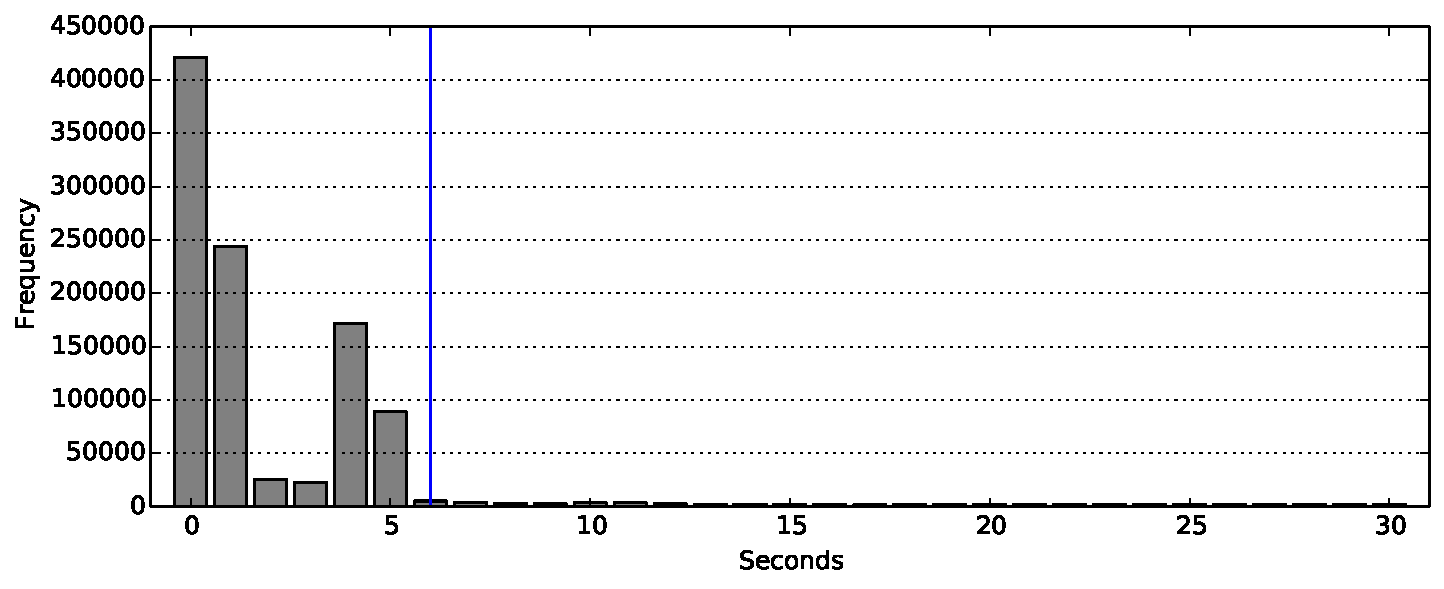
\includegraphics[width=\textwidth]{graphics/2015-08-14_17-46-44_faui1-246_timeout}
\caption{Duration of receiving one peer message}
\label{timeout-calibration}
\end{figure}

To assess a minimum timeout, an analysis with special configuration parameters was performed\footnote{Files: \texttt{2015-08-14\_17-46-44\_faui1-246.sqlite}, \texttt{2015-08-14\_17-46-44\_faui1-246\_timeout.txt}}. Here the maximum time used for receiving one message was recorded for every peer contact. These durations were rounded and the number of occurrences plotted in figure \ref{timeout-calibration}. For this task \config{network\_timeout} was set to 30 seconds to achieve most unbiased results. During this test at \numprint{977301} out of \numprint{1040817} peer contacts the maximum duration for receiving one message was below six seconds, which equals \numprint[\%]{93.9}.

\paragraph{\config{torrent\_complete\_threshold}}
\dots

\paragraph{\config{peer\_evaluation\_threads}}
\dots

TODO: Number of threads: workload plot

\begin{figure}
\centering
%\includegraphics[width=\textwidth]{graphics/2015-08-20_11-52-13_faui1-246_workload}
\caption[Load parameters during the analysis]{a and b}
\label{load}
\end{figure}

\section{Restrictions}

Restrictions and why this does not invalidate the results (hopefully, TBD):

\begin{itemize}
  \item No support for IPv6 on HTTP, UDP or DHT requests
  \item No support for the Micro Transport Protocol ($\mu$TP)
  \item No support for Peer exchange (PeX)
  \item No support for the Tracker exchange extension (BEP 28)
  \item No support for the BitTorrent Local Tracker Discovery Protocol (BEP 22)
  \item No BitTrorrent Protocol support for getting download progress info
  \item Drawback: One can only derive lower bounds from observing peers using the standard BitTorrent protocol
\end{itemize}


\section{Usage}
pymdht: It must me started seperately and is controlled automatically using a localhost Telnet connection. It could not be integrated directly, since it is written in Python version 2. The desired UDP node port and the Telnet control port must be given as arguments and should reflect the values written in the \emph{BitTorrent Download Analyzer's} configuration file. The typical command used here is \texttt{run\_pymdht\_node.py -{}-port=17000 -{}-telnet-port=17001}. It is sensible to check whether \emph{pymdht} has crashed before and after each analysis run to ensure complete results.

The main script, named \texttt{btda.py} can be controlled by using the following command line options.

\begin{description}
  \item[\texttt{-{}-active <threads>}] Actively contact and evaluate peers using the specified number of threads.
  \item[\texttt{-{}-passive}] Listen on the port specified in the configuration file for incoming connections and evaluate these peers.
  \item[\texttt{-{}-dht}] Integrate and control an already running \emph{pymdht} \cite{pymdht} DHT node using Telnet. The UDP port on which the node is running and the localhost Telnet port where \emph{pymdht} can be controlled are given via \config{dht\_node\_port} and \config{dht\_control\_port} respectively.
  \item[\texttt{-{}-debug}] Write log messages to the console instead of a file and include debug messages.
  \item[\texttt{-{}-help}] Show a help message and exit.
\end{description}
%%%%%%%%%%%%%%%%%%%%%%%%%%%%%%%%%%%%%%%%%%%%%%%%%%%%%%%%%%%%%%%%%%%%%%%%%%%%%%%%%%

\chapter{Evaluation}
Data collection with the BitTorrent Download Analyzer tool was performed on a virtual machine running Ubuntu 14.04 LTS with 1.0\,GB of RAM, a 3.4\,GHz processor and an own IPv4 address without NAT. The 15 chosen torrents were analyzed at once concurrently using \textbf{512 threads}. The analysis was performed \range. A time period of \textbf{48 hours} was chosen in order to detect patters during the day-night cycle. Necessary measures to ensure valid results were taken: The DHT node provided by \emph{pymdht} did not crash before or during the analysis. The BitTorrent Download Analyzer or any of its threads did not crash during the analysis and gave no relevant error message in the logfile.

[Thread workload and system load were normal as described earlier*.]

\section{Choosing Torrents}
\begin{table}
\centering
\begin{tabular}{rllr}
\toprule
Rank & Site name & Domain name & Alexa Rank \\
\midrule
1 & Kickass Torrents & \texttt{kat.cr} & 116 \\
2 & ExtraTorrent.cc & \texttt{extratorrent.cc} & 335 \\
3 & Nyaa Torrents & \texttt{www.nyaa.se} & 399 \\
4 & Torrentz Search Engine & \texttt{torrentz.eu} & 464 \\
5 & The Pirate Bay & \texttt{thepiratebay.se} & 507 \\
6 & YTS & \texttt{yts.to} & 669 \\
7 & Rarbg & \texttt{rarbg.to} & 1,150 \\
8 & 1337x & \texttt{1337x.to} & 1,661 \\
9 & EZTV & \texttt{eztv.ch} & 1,831 \\
10 & torrentHound.com & \texttt{www.torrenthound.com} & 2,188 \\
11 & IPTorrents & \texttt{iptorrents.com} & 3,256 \\
12 & isoHunt & \texttt{isohunt.to} & 3,816 \\
13 & Bitsnoop P2P Search & \texttt{bitsnoop.com} & 4,293 \\
14 & Torrent Downloads & \texttt{www.torrentdownloads.me} & 4,315 \\
15 & LimeTorrents.cc & \texttt{www.limetorrents.cc} & 4,552 \\
16 & TamilRockers.net & \texttt{tamilrockers.com} & 4,586 \\
17 & Monova Torrent Search & \texttt{www.monova.org} & 4,843 \\
\bottomrule
\end{tabular}
\caption[Popular torrent directory sites according to \textsc{Alexa}]{Popularity of torrent directory sites according to \textsc{Alexa}'s \cite{alexa} global traffic ranking. Only sites with a rank below \numprint{5000} are listed. Data is accurate as of July 16, 2015.}
\label{torrentsites}
\end{table}

Due to the distributed nature of BitTorrent, there unfortunately is no complete list or for all torrents currently active. Thus external data about popularity of torrents is needed, even if there is no guarantee of correctness. So to determine most popular torrent directory sites the global traffic rankings by \textsc{Alexa Internet, Inc.} \cite{alexa} were consulted. The websites where \textsc{Alexa}'s ranking was looked up were collected through manual investigation using web search engines, relevant news sites and cross references between torrent sites. Table~\ref{torrentsites} shows the \numprint{17} sites found having an rank below \numprint{5000}.

\begin{table}
\centering
\begin{tabular}{lrlrrr}
\toprule
Set & ID & Torrent name & Size & Leechers & Seeders \\
\midrule
A & 1 & torrent\_name & 3.0\,GB & 42 & 23 \\
& 4 & torrent\_name & 3.0\,GB & 42 & 23 \\
& 8 & torrent\_name & 3.0\,GB & 42 & 23 \\
& 11 & torrent\_name & 3.0\,GB & 42 & 23 \\
& 13 & torrent\_name & 3.0\,GB & 42 & 23 \\
B & 3 & torrent\_name & 3.0\,GB & 42 & 23 \\
& 6 & torrent\_name & 3.0\,GB & 42 & 23 \\
& 9 & torrent\_name & 3.0\,GB & 42 & 23 \\
& 10 & torrent\_name & 3.0\,GB & 42 & 23 \\
& 14 & torrent\_name & 3.0\,GB & 42 & 23 \\
C & 5 & torrent\_name & 3.0\,GB & 42 & 23 \\
& 7 & torrent\_name & 3.0\,GB & 42 & 23 \\
& 12 & torrent\_name & 3.0\,GB & 42 & 23 \\
& 15 & torrent\_name & 3.0\,GB & 42 & 23 \\
& 16 & torrent\_name & 3.0\,GB & 42 & 23 \\
\bottomrule
\end{tabular}
\caption[List of torrent chosen for evaluation]{* List of the 20 most popular torrents according to meta-search engine \textsc{Torrentz} \cite{torrentz}. At the end are five torrents above \numprint[GB]{5} and five recently published torrents . Selection was made on August 42, 2015, 11:00. The \emph{ID} was chosen by the SQLite database used for storage during the analysis.}
\label{torrents}
\end{table}

Popular torrents were often found to be registered on multiple tracker sites, which leads to mostly identical top torrents across various torrent sites. For the definite selection of torrents, the meta-search engine \textsc{Torrentz} \cite{torrentz} was used: It monitors torrents from all other major torrent sites and provides sort and filter options by peer count, torrent age and size. Torrents in three size groups were chosen:

\begin{itemize}
  \item Set A: The 8 most popular torrents below \numprint[GB]{1} % (1,4,8,11,13)
  \item Set B: The 8 most popular torrents above \numprint[GB]{1} % (3,6,9,10,14)
  \item Set C: The 8 most popular torrents above \numprint[GB]{10} % (5,7,12,15,16)
\end{itemize}

Popular torrents were chosen regarding leecher numbers, despite the website sorting by the sum of seeders and leechers. Set B only contains only torrent smaller than \numprint[GB]{10} since larger torrents are less pupular in comparision. The 27 chosen torrents are listed in table \ref{torrents}. These three sets will be evaluated separately where appropriate.

\section{Getting Addresses of Peers}
\begin{table}
\centering
\begin{tabular}{lrrrr}
\toprule
Source & Total & Unique & New & Unique per Hour \\
\midrule
Tracker server & 5 & 2 & 3\,\% \\
DHT network & 10 & 2 & 3\,\% \\
Incoming peers & 1 & 2 & 3\,\% \\
\bottomrule
\end{tabular}
\caption[Received peer addresses per source]{Total and unique received peer \textbf{addresses} per source. \emph{Tracker server} and the \emph{DHT network} are actively contacted for new peers. Values of \emph{incoming peers} only include peers whose download progress was evaluated successfully. The duration to calculate the \emph{unique per hour} value is \numprint[h]{48}*, as mentioned earlier.}
\label{unique-peers}
\end{table}

Peers from all sources were considered, namely from the tracker server, the DHT network and incoming connections. The total number collected across all torrents during this analysis in regards to their source is shown in table \ref{unique-peers}. Since the \emph{incoming peers} data point in this table only includes peers when their download progress was successfully evaluated, the ratio of \numprint[\%]{95}* new incoming peers implies that $1-\numprint[\%]{95}=\numprint[\%]{5}$* of unique incoming peers contacted us a second time, despite not receiving any torrent data.

\begin{figure}
\centering
\includegraphics[width=\textwidth]{graphics/2015-08-19_20-43-43_faui1-246_source_all_torrents}
\caption[Development of received peer addresses per source]{Development of received peer \textbf{addresses} per source for all torrents, on average. New peers from the tracker server and the DHT network are requested every five minutes. UDP trackers returned always \numprint{200} addresses per request, trackers with HTTP access \numprint{50}. Torrents are usually registered with few trackers. DHT request were observed to return between \numprint{100} and \numprint{1300} peers each. The values \emph{incoming-unique} and \emph{incoming-duplicate} only include peers after their download progress was extracted successfully. The analysis lasted \range.}
\label{request-history}
\end{figure}

The progression of received peer addresses during the analysis period is shown in figure \ref{request-history}. Again, this is a summary for all torrents. From the incoming peers, only the ones represented by \emph{incoming-duplicate} are candidates to be counted as confirmed downloads, since the were evaluated at least twice. The ratio between new and duplicate received peer address information is slightly higher in the first hours*.

[In general the amount of duplicate received peers is above xx\%*, so presumably many of the addresses known to trackers and the DHT network are collected in this process.]

\section{Counting Confirmed Downloads}
\begin{table}
\centering
\begin{tabular}{lrrrr}
\toprule
Torrent & Confirmed & Reported & Confirmed/Reported & Unique Peers \\
\midrule
Set A & 5 & 2 & 3\,\% \\
Set B & 10 & 2 & 3\,\% \\
Set C & 1 & 2 & 3\,\% \\
\bottomrule
\end{tabular}
\caption[Confirmed downloads per torrent set]{Confirmed \textbf{downloads} per torrent set. In comparison, \emph{reported} downloads are responses from scrape requests to the tracker during the analysis. \emph{Unique peers} are all peers successfully evaluated for the torrents in question, although not crossing the confirmed download threshold.}
\label{confirmed-downloads}
\end{table}

Table \ref{confirmed-downloads} shows the confirmed download numbers measured during this analysis per torrent set. For comparison, numbers reported by the tracker in scrape requests are given. * [Compare sets and unique peers]

[Note all things in the plots, even the obvious] Scrape is higher than confirmed.

[downloaded (event=complete) vs complete (seeders), \cite{watters2011much} uses seeders]

[try different thresholds]

\begin{figure}
\centering
\includegraphics[width=\textwidth]{graphics/2015-08-20_11-52-13_faui1-246_download_set_(1,4,8,11,13)}
\includegraphics[width=\textwidth]{graphics/2015-08-20_11-52-13_faui1-246_download_set_(3,6,9,10,14)}
\includegraphics[width=\textwidth]{graphics/2015-08-20_11-52-13_faui1-246_download_set_(5,7,12,15,16)}
\caption[Development of confirmed and reported downloads per torrent set]{Development of \emph{confirmed} and server reported \textbf{downloads} per torrent set. From top to bottom: Set A ($<\numprint[GB]{1}$), set B (\numprint[GB]{1} to \numprint[GB]{10}) and set C ($>\numprint[GB]{10}$). Server reported numbers are gathered using \emph{scrape} requests. Analysis duration was \range.}
\label{download-history}
\end{figure}

The history of download numbers during the analysis period is shown in figure \ref{download-history}.

[Check single torrents for outliers]

[correlation with scrape bachelor and ieee bt]

\subsection{Problems of this Method}
\label{problems}
\begin{table}
\centering
\begin{tabular}{llrr}
\toprule
Event & Error & Quantity & Share per Event \\
\midrule
First contact & timed out & 182209 & 63.8\% \\
& Socket connection broken & 47690 & 16.7\% \\
 & Connection refused & 47028 & 16.5\% \\
 & No route to host & 4938 & 1.7\% \\
 & Connection reset by peer & 3330 & 1.2\% \\
 &  Network is unreachable & 213 & 0.1\% \\
 & Peer speaks unknown protocol & 5 & 0.0\% \\
 & \textit{Total} & 285413 &  \\
\midrule
Later contact & Socket connection broken & 3847 & 55.9\% \\
 & timed out & 2244 & 32.6\% \\
 &  No route to host & 369 & 5.4\% \\
 & Connection refused & 249 & 3.6\% \\
 &  Connection reset by peer & 176 & 2.6\% \\
 & \textit{Total} & 6885 &  \\
\midrule
Incoming peer & Unknown info hash & 399331 & 68.3\% \\
 & Peer speaks unknown protocol & 124794 & 21.4\% \\
 & timed out & 57021 & 9.8\% \\
 & Connection reset by peer & 1821 & 0.3\% \\
 & Socket connection broken & 1427 & 0.2\% \\
 & \textit{Total} & 584394 &  \\
\bottomrule
\end{tabular}
\caption[Reasons for failure of peer evaluation]{Outcome of peer evaluations during the analysis process with error and success rates. \emph{Event} describes the point in the evaluation process, when the problem occurred. \emph{First} and \emph{later contact} are performed when actively contacting collected peer addresses, while a peer must be contacted once successfully to be contacted another time. An \emph{incoming peer} represents an incoming connection on the BitTorrent listening port.} % TODO* add success (maybe all_incoming_peers, unique success)
\label{connection-failure}
\end{table}

The Evaluation of a peer's download progress was described in section \ref{peer-evaluation}. This process can fail for various reasons. The superficial problems which occurred in this analysis are listed in table \ref{connection-failure}. The table shows every attempt of connecting to a peer and performing the evaluation procedure. Outgoing evaluation attempts were usually* successful. The mainly* appearing error is a timed out peer, which indicates outdated or wrong peer address information. However, the value of failed evaluations on a second or later contact is very low. Regarding incoming peers, most evaluations* failed due to an unknown info hash. This is probably because of other torrents evaluated beforehand from the same IP address and port. The response rate between peers obtained via trackers and peers received through the DHT network was not examined.

The search for more fundamental explanations for errors merely speculation. Peers may blacklist the IP of the analysis program over time, since the don't receive any data at all. Also, peers could only support the UDP based Micro Transport Protocol ($\mu$TP), which is not supported by this analysis tool. When peers have no free upload capacity, they may block all incoming connections. When the evaluation on a peer failed once, no second try will be made. If this only happens due to a temporary network problem and the peer is in fact downloading, this will not be noticed. Presumably the biggest problem are BitTorrent clients without an exposed port, in other words peers behind a NAT. Since this is the case with a computer behind a standard home router, this setup is very common. Several of these machines will connect to our program after receiving our IP address from a tracker or the DHT network*, but there is no guarantee to capture all of them. Finally, the BitTorrent client could be terminated immediately after the download finished, leaving no time for us to register any further progress.

\section{Peers Analysis}
\subsection{Download Speed}
filter peers for visits

filter countries for peers

TODO: Graph of speed per country with standard derivation indicators, n>=10 per country

todo: Map of Distribution of download speeds

Map: Distribution of downloads (TODO)

\subsection{BitTorrent Clients}
\label{clients}
TODO: Table of frequency of BT clients

\subsection{Peer's Host Names}
TODO: Table: Examine hostnames by ISP or seedbox provicers
%%%%%%%%%%%%%%%%%%%%%%%%%%%%%%%%%%%%%%%%%%%%%%%%%%%%%%%%%%%%%%%%%%%%%%%%%%%%%%%%%%

\chapter{Conclusion and Future Work}
\dots
%%%%%%%%%%%%%%%%%%%%%%%%%%%%%%%%%%%%%%%%%%%%%%%%%%%%%%%%%%%%%%%%%%%%%%%%%%%%%%%%%%

\printbibheading[heading=bibintoc]
\begingroup
\setlength\labelnumberwidth{0.57cm}
\printbibliography[heading=subbibintoc, title={Research}, keyword=science]
\printbibliography[heading=subbibintoc, title={Software}, keyword=software]
\printbibliography[heading=subbibintoc, title={Online}, keyword=online]
\printbibliography[heading=subbibintoc, title={Other}, notkeyword=science, notkeyword=standard, notkeyword=software, notkeyword=online] % TODO: remove, should be empty *
\endgroup
\printbibliography[heading=subbibintoc, title={Standards}, keyword=standard]
\end{document}
